%!TEX root = ../dissertation.tex
%\begin{savequote}[75mm]
%This is some random quote to start off the chapter.
%\qauthor{Firstname lastname}
%\end{savequote}

\chapter{Dataset}
\label{dataset}

In this chapter it will be presented the dataset that has been utilized for this work. As previously mentioned, the main focus is asked to be Italian automotive forums, so the first phase consisted in the search of reliable resources from which retrieve the needed information. Data gathering has been made by crawling the founded web forums. After getting all the information, the final phase for what concerns the dataset consists on annotate all the forums' comments on the base of diverse topics. \\
In the following sections the whole procedure has been presented in detail.

\section{Dataset Retrieval}

Sentiment analysis is a practical natural language processing problem, most commonly faced involving machine learning techniques. As discussed in detail in Chapter 2, machine learning algorithms need a set of labeled data that represent the environment where the algorithm is supposed to work on. As good sampled data represent the true data distribution, as good the model should work on the real environment, so the dataset retrieval is fundamental for the final outcomes.\\
This work is focused on Italian automotive forums, so the first important phase is to identify some reliable resources where to extrapolate the needed information. 


\subsection{Forums' List}

Web forums are websites (or sections of websites) that allow visitors to communicate with each other by posting messages. Most forums allow anonymously visitors to view forum contents, except for registration-required ones. Forums are available for all kinds of topics, from software to health, and like in this case, automotive. Forums are composed by user-generated content, so they are full of users' opinions then, as just mentioned, they are good environments to acquire datasets for sentiment analysis. Forums are commonly subdivided in "areas" or "rooms" which are thematic macro partitions. Rooms are again subdivided into "sections", which are discussions' categories belonging to the same thematic area. Finally, sections contain numerous "threads", which are the actual discussions.\\



For this work, target resources are identified in Italian automotive web forums or blogs with possibility of discussion, with an active community. The identified resources are: Quattroruote(\url{https://forum.quattroruote.it/}), Autopareri (\url{https://www.autopareri.com/forum}), Bmwpassion (\url{https://www.bmwpassion.com/forum/}), Porschemania (\url{http://www.porschemania.it/discus/}) and HDmotori (\url{http://www.hdmotori.it/}). 
%Some statistics are summarized in Table \ref{table:forum-list}.



%\begin{table}[ht]
%	\renewcommand{\arraystretch}{2.5}
%	\centering
%	\begin{tabular}{| >{\centering\bfseries}m{3cm} | >{\centering}m{1in} | >{\centering}m{1in} | >{\centering}m{1in} | >{\centering\arraybackslash}m{1in} | } 
%		\hline
%		\textbf{Resource} & \textbf{Type} & \textbf{\# Threads} & \textbf{\# Messages} & \textbf{\# Users} \\ [.2cm]
%		\midrule
%		Quattroruote & Forum & 121,366 & 2,413,452 & 70,707 \\ [.2cm]
%		\hline
%		Autopareri & Forum & n.a & 2,146,532 & 34,963 \\ [.2cm]
%		\hline
%		Bmwpassion & Forum & 349,259 & 7,909,297 & 78,608
%		 \\ [.2cm]
%		\hline
%		Porschemania & Forum & n.a & n.a & n.a \\ [.2cm]
%		\hline
%		HDmotori & Blog & n.a. & n.a. & n.a. \\ [.2cm]
%		\hline
%	\end{tabular}
%	\caption{Forums' statistics updated in date 15/08/2019.}
%	\label{table:forum-list}
%\end{table}



% TODO eventualmente spiegare qualcosa di tutti i forum

All resources except for Porschemania are brand independent, which means that are treated discussions about every automotive brands independently, while the last one is focused on Porsche \footnote{Porsche is a German sports car manufacturer located in Zuffenhausen in Stuttgart, founded in 1931 by Ferdinand Porsche.} discussions.\\
The dataset will be composed as a list of comments, so the idea is to download as mush information as possible, that is common to each resource, in order to represent precisely the environment in a structured way like a \ac{CSV} file.

\subsection{Comments' Information}

Forums can be seen as a temporal ordered list of comments grouped into discussion. In this way the core part of representing discussions passes through the comment representation. Actually, it is irrelevant the way on which represent the information, but it is fundamental decide what information to keep. An idea is to keep all possible information common to comments of all resources, in order to even all entries in a standard way. In Figures \ref{fig:screen-quattroruote} \ref{fig:screen-autopareri} \ref{fig:screen-porschemania} \ref{fig:screen-bmwpassion} \ref{fig:screen-hdmotori} are shown one comment for each of the selected resources, with highlighted the information that have been decided to be extracted.

\begin{figure}[!hb]
	\centering
	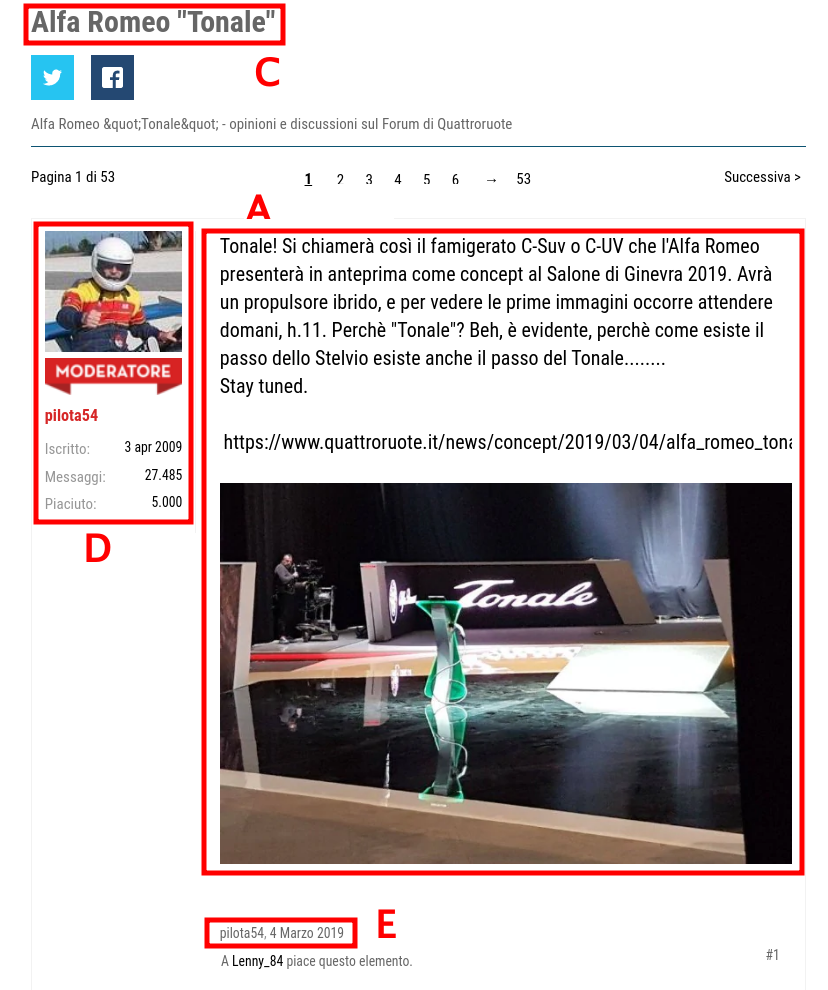
\includegraphics[width=1\textwidth]{figures/screen/screen-quattroruote.png}
	\caption{Sample comment in Quattroruote's forum}
	\label{fig:screen-quattroruote}
\end{figure}

\begin{figure}[!htb]
	\centering
	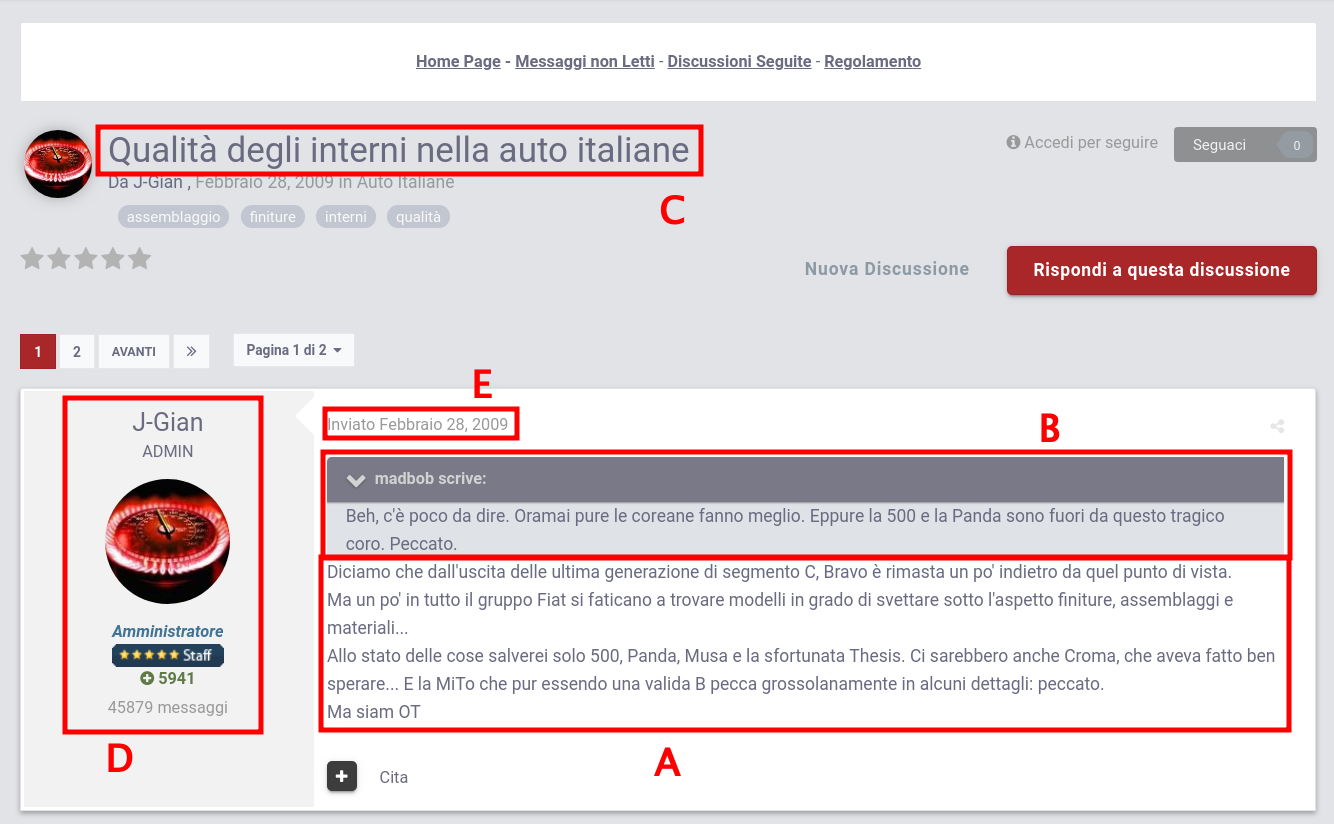
\includegraphics[width=1\textwidth]{figures/screen/screen-autopareri.png}
	\caption{Sample comment in Autopareri's forum}
	\label{fig:screen-autopareri}
\end{figure}

\begin{figure}[!htb]
	\centering
	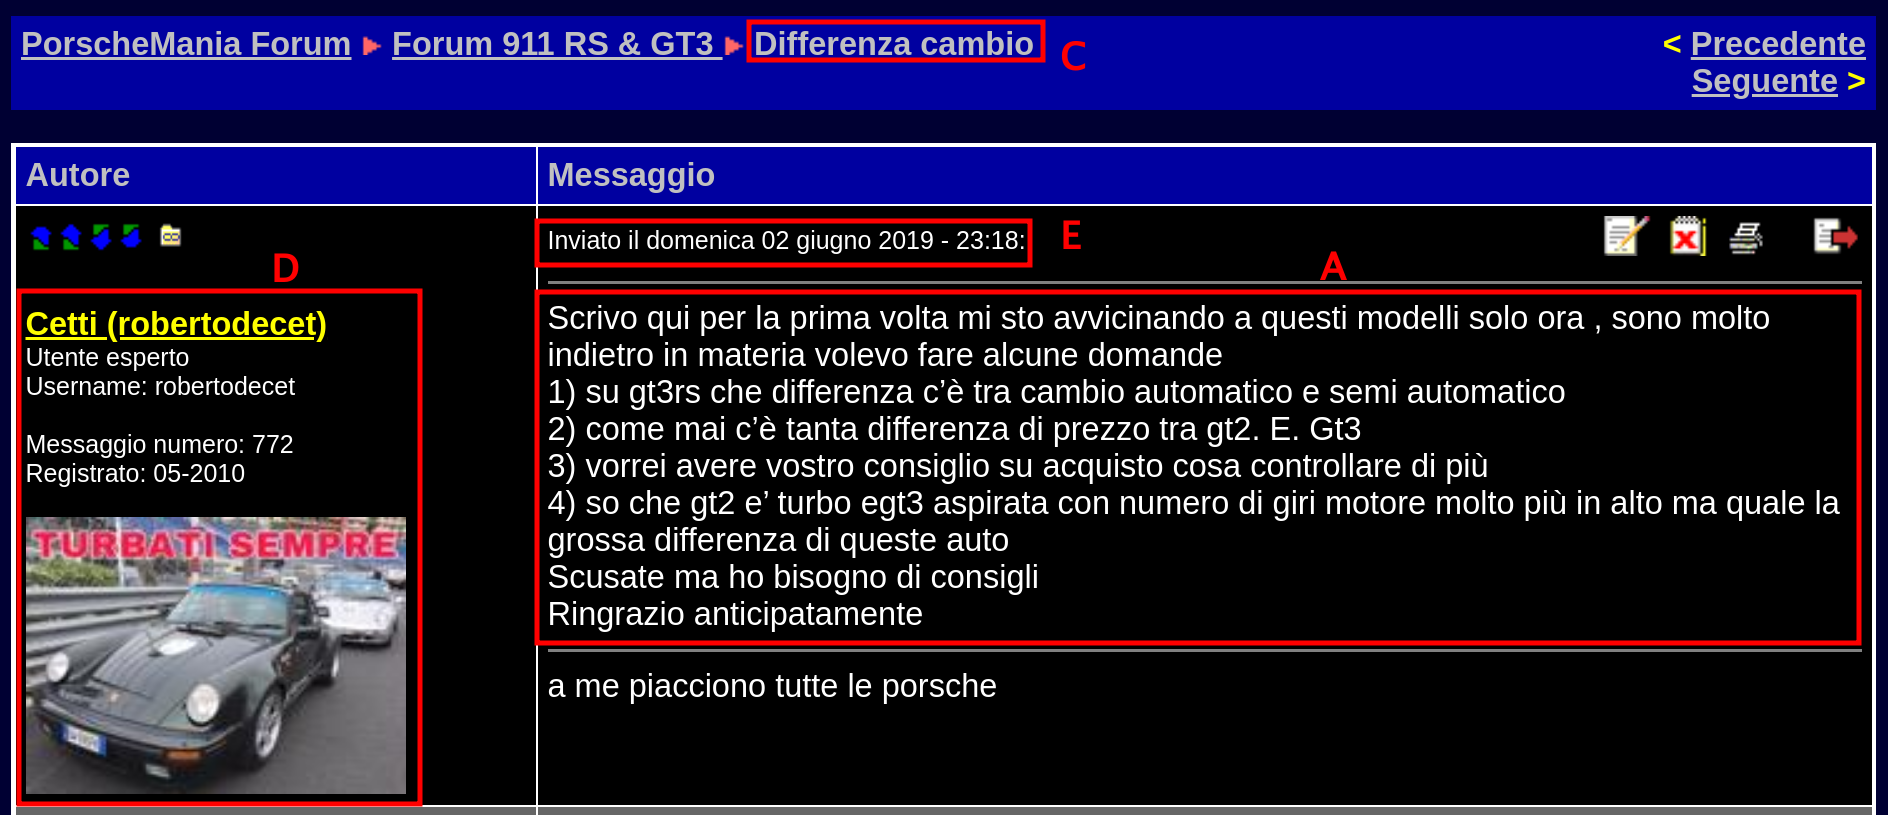
\includegraphics[width=1\textwidth]{figures/screen/screen-porschemania.png}
	\caption{Sample comment in Porschemania's forum}
	\label{fig:screen-porschemania}
\end{figure}

\begin{figure}[!htb]
	\centering
	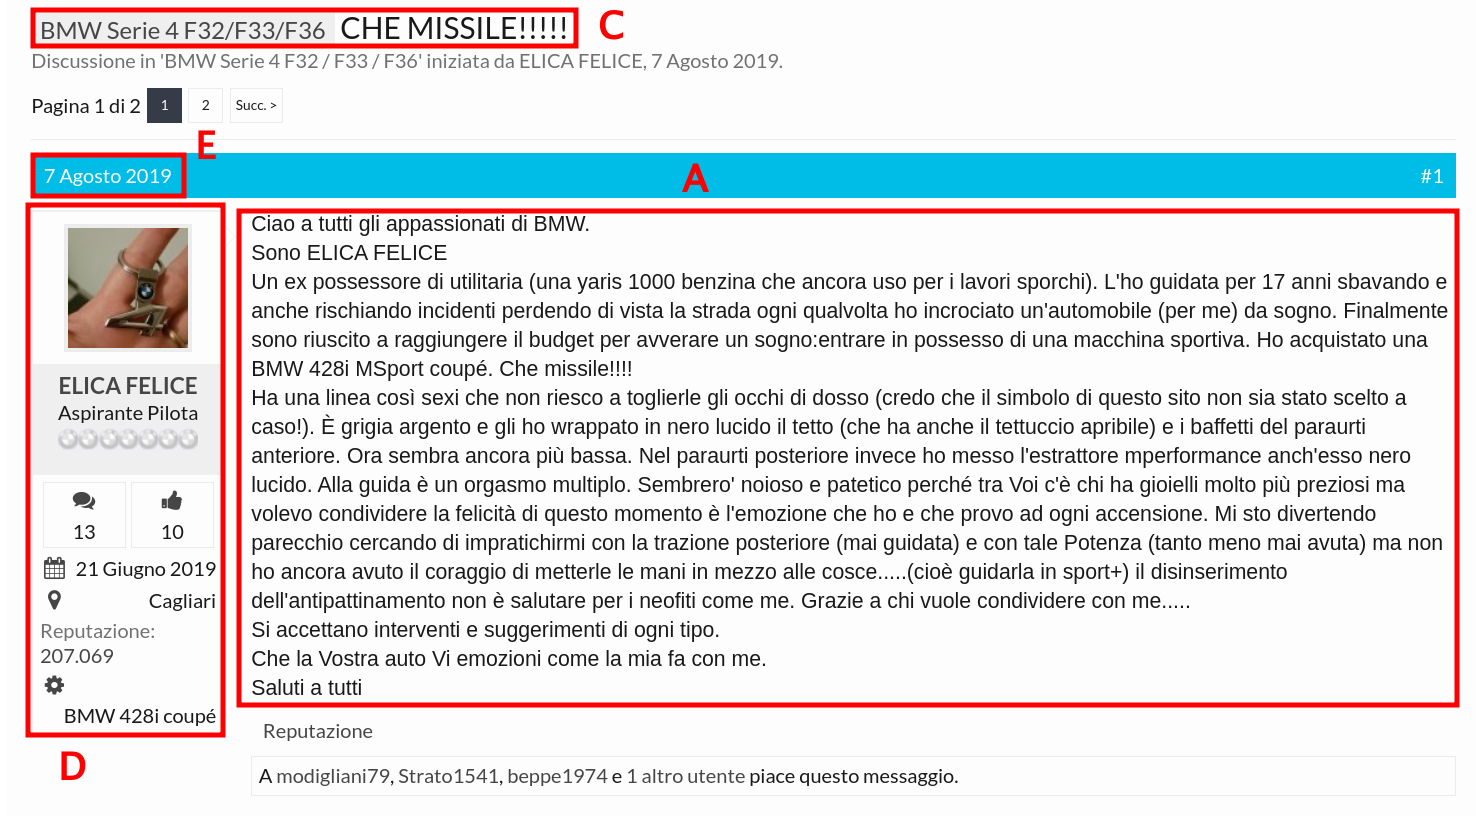
\includegraphics[width=1\textwidth]{figures/screen/screen-bmwpassion.png}
	\caption{Sample comment in Bmwpassion's forum}
	\label{fig:screen-bmwpassion}
\end{figure}

\begin{figure}[!h]
	\centering
	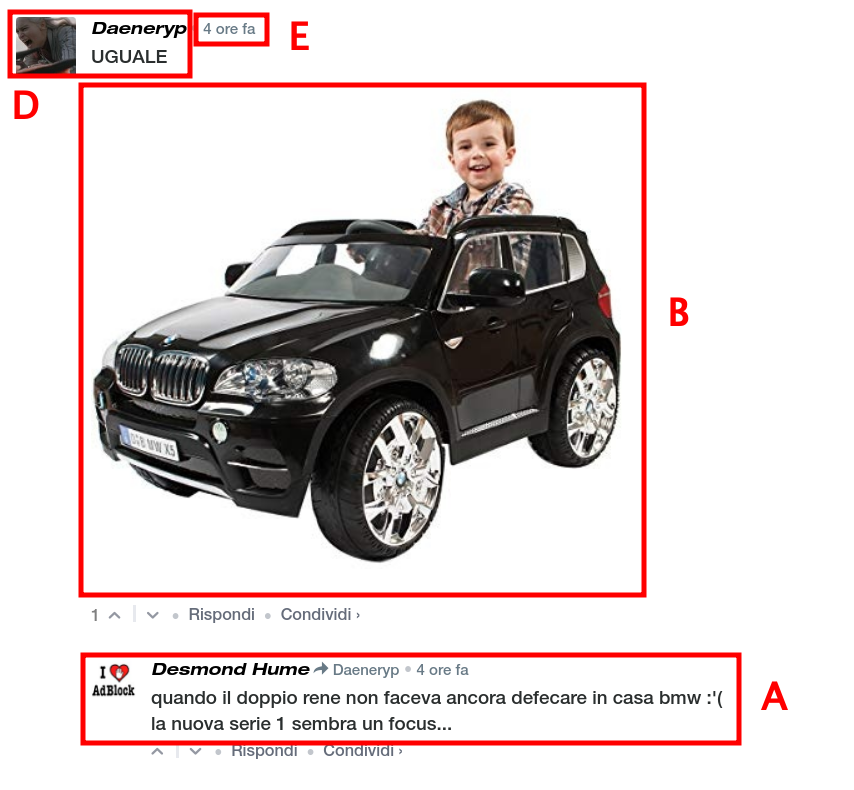
\includegraphics[width=1\textwidth]{figures/screen/screen-hdmotori.png}
	\caption{Sample comment in HDmotori's blog}
	\label{fig:screen-hdmotori}
\end{figure}

The highlighted information are summarized in the following items. The letter is the reference of the square in the image (not every item is shown because of page dimension):

\begin{itemize}
	\item \textbf{Text (A)}: the text of the comment. It is the most important information about the comment;
	
	\item \textbf{Quote (B)}: some comments may reference another user's comment in the discussion. This citation is an important information because it gives context about the text of the entry;
	
	\item \textbf{Topic's Title (C)}: the main title of the discussion;
	
	\item \textbf{Author (D)}: the username of the user that wrote the comment;
	
	\item \textbf{Comment's Timestamp (E)}: all comments contain temporal information about when they are written.
\end{itemize}


\subsection{Information Gathering}

All information needed are viewed in web pages, but they are not accessible from any API or some other data storage interface. For this reason the only solution is to crawl all discussions' web pages and extract the information we need by parsing the \ac{HTML} file (\ac{HTML} scraping). \\
The following paragraphs explain all information and processes used to obtain the desired data explained earlier.

\subsubsection{HTML Structure}

Web pages are written in \ac{HTML}, that is a markup language designed by Tim Berners Lee in 1993. It is the standard markup language designed to be displayed in web browsers. HTML was delivered in several version: \ac{HTML} 2 comes in 1995, \ac{HTML} 3 in 1997, \ac{HTML} 4 in 1997 and the nowadays version HTML 5 in 2014. \\
As a markup language it is composed by textual information tagged by \ac{HTML} markups. A markup consists of tags which appear inside angled brackets  like "< tag >", that give information about how text should be formatted in a browser.	Most of the \ac{HTML} elements are composed by two actual tags: an opening tag <tag> and a closing tag </tag>. Each element may contain other elements and so on, making \ac{HTML} structured as a tree. Although several HTML markups have been introduced, a correct HTML document must always include certain tags following the standard structure:

\begin{center}
\begin{lstlisting}
<!DOCTYPE html>
<html>
   <head>
      <title>This is a title</title>
   </head>
   <body>
      <p>Hello world!</p>
   </body>
</html>
\end{lstlisting}
\end{center}

The web page content is included into the <body> tag. \\
Some commonly used HTML tags are the followings (in alphabetical order):
\begin{itemize}
	\item <!-- -->: used to define a comment that is ignored by the browser;
	\item <!DOCTYPE html>: tells the browser what kind of document it is loaded;
	\item <a>:  used to define an anchor (or hyperlink);
	\item <article>: used to contain blog entries;
	\item <b>: used to formatting the text bold;
	\item <blockquote>: used for quoting an external source;
	\item <body>: defined the body of the HTML document;
	\item <br>: single line break;
	\item <button>: defines a button that can be clicked;
	\item <caption>: used to define the table's caption;
	\item <div>: defines a container;
	\item <dl>: description list, items into <dd> or <dl> tags;
	\item <form>: forms for user inputs;
	\item <h1>, <h2>, ... , <h6>: defines headings. Lower is the number, higher is the level of the heading;
	\item <head>:  head section of the document, used for metadata;
	\item <header>: contains content to be displayed on top of the body;
	\item <html>: the root of the document. All tags must be inside this tag;
	\item <img>: displays an image;
	\item <input>: used to create forms input elements;
	\item <ol>: ordered list, items in to <li>;
	\item <style>: used for declaring inline style;
	\item <ul>: unordered list, items into <li>.
\end{itemize}

Clearly, an \ac{HTML} document is a composition of all these (and other) tags, that when put together, create into the web browser a readable webpage that displays some content. Moreover, all (or almost all) \ac{HTML} tags can have attributes that provide additional information about elements, specifying those in the format attribute="value" inside the start tag. This is used, for instance, in <a> tag to specify the hyperlink reference, such as:
\begin{lstlisting}
<a href="https://www.unipd.it">This is a link</a>
\end{lstlisting}
Important attributes are  "id" and "class". The value of the attribute "id"  must be unique on the entire document, while more elements can have the same value of the attribute "class". These attributes are used as selectors, for instance for defining the style or the behavior, but since it is not relevant for what concerns the data crawling strategy, it will be not covered in detail.\\


\subsubsection{HTML Parser}

HTML documents, for their nature of tree structure, can be accessible by \ac{DOM} \ac{API}. \ac{DOM} is a platform-independent and language-independent object model for HTML (and other markup languages) documents. It allows programs and scripts to dynamically access and update the content, structure and style of the document \cite{html-dom}. It describes the objects (identified as nodes) that compose the entire document structure and the interfaces to be accessed and manipulated by programs. Using \ac{DOM} is possible to read, create and modify \ac{HTML} documents dynamically. An example of \ac{DOM} of a simple HTML document is shown in Figure \ref{fig:html-dom}.

\begin{figure}[ht]
	\centering
	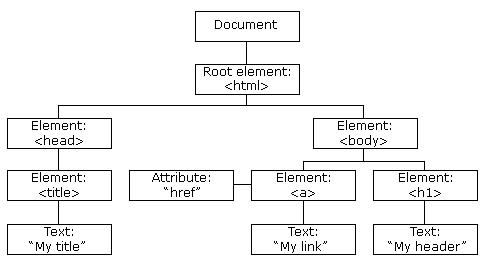
\includegraphics[width=1\textwidth]{figures/html-dom.png}
	\caption{Graphical representation of an HTML DOM}
	\label{fig:html-dom}
\end{figure}

\ac{DOM} implementations create an in-memory representation of the \ac{HTML} tree, where each element with its attributes is represented with a node. Each node has children nodes that represent the inner elements of the parent, and so on. Starting from the initial <html> tag, referenced as the root of the tree, it is possible to build the entire structure.\\

In Python language, "Beautiful Soup" (\url{https://www.crummy.com/software/BeautifulSoup/}) is a library that implements the \ac{DOM} interface for \ac{HTML} documents. It provides a simple interface to parse a \ac{HTML} document, in order to get the needed information. Since for retrieving forums' information there are not available resources, the only solution is to parse \ac{HTML} web pages, understand where the needed information are located (which actually means find the exact tags where they stand), and finally get them using the given \ac{API}. Since real web pages have a complicate structure, it is helpful to exploiting browsers'  inspector tools. With Beautiful Soup it is possible to query tags by name, by relationship with other tags (for instance, get all children of a given tag), or by attribute. An example of query that retrieves all <p> tags from an \ac{HTML} document is shown in Listing \ref{lst:html_query_p}.

\lstset{language=Python}
\lstset{frame=lines}
\lstset{caption={Example of a query in a HTML document with BeautifulSoup}}
\lstset{label={lst:html_query_p}}
\lstset{basicstyle=\footnotesize}
\begin{lstlisting}
from bs4 import BeautifulSoup

# suppose html is a HTML document
soup = BeautifulSoup(html, 'html.parser')
soup.find_all('p')

# it returns a list of <p> tags, like
# [<p>Hi, my name is</p>, <p>John</p>, <p>Live in SF</p>]
\end{lstlisting}



\subsubsection{Crawler}

Crawling is the process of automatically browsing the World Wide Web (or an interested part of it) using some programmed scripts called \textit{crawlers}. This process is commonly used by search engines form indexing web pages.\\
World Wide Web, or in a lower scale a single website, can be viewed as a directed graph where every page contain links to other pages. While viewing web as a directed graph, web pages can be considered as nodes, and hyperlinks can be considered as edges. In this way it is possible to summarize search operations (and obviously also web crawling) as traversing a directed graph \cite{article-web-crawling}. Web crawlers are designed to automatically retrieve information from visited pages.\\
The working of web crawlers starts with an initial set of URLs, known as \textit{seeds}, then it downloads all these web pages and extracts new links present in the page, eventually filtering out some irrelevant ones. The downloaded pages are then processed and all extracted information are stored. This process, summarized in Figure \ref{fig:web-crawler}, continues recursively until there are no more URLs to be visited. 

\begin{figure}[ht]
	\centering
	
\includegraphics[width=0.6\textwidth]{figures/web-crawler.png}
	\caption{Web Crawling process}
	\label{fig:web-crawler}
\end{figure}

In this work, for simplicity, have been implemented two different web crawlers for each forum: the first one is supposed to extract all base discussion links starting from a set of manually selected seeds, which are the main pages of thematic areas, while the second is asked to crawl every entire discussion, starting from the previously found URLs. The main structures of the two crawlers are shown in Algorithms \ref{alg:crawler-1} \ref{alg:crawler-2}, which actually implement a sort of \ac{DFS} traversal algorithm. Page downloading is performed using the "urllib" Python library (\url{https://docs.python.org/3/library/urllib.html}).

\begin{algorithm}
	\caption{Crawler for discussions' base links retrieval}
	\label{alg:crawler-1}
	\begin{algorithmic}[1]
		\State \textbf{initialize} seeds =[set of thematic areas' links], urls = []
		\State
		\While {seeds is not empty}
		\State url = seeds.pop()
		\State next = "next page link"
		\For{discussion link d in current page}
		\State urls.enqueue(d)
		\EndFor
		\State seeds.push(next)
		\EndWhile
		\State \textbf{return} urls
	\end{algorithmic}
\end{algorithm}

\begin{algorithm}
	\caption{Discussions' Crawler}
	\label{alg:crawler-2}
	\begin{algorithmic}[1]
		\State \textbf{initialize} comments = []
		\State
		\State seeds = result from Algorithm \ref{alg:crawler-1}
		\While {seeds is not empty}
		\State next = "next page link"
		\For {comment c in current page}
		\State comments.enqueue(c)
		\EndFor
		\State seeds.push(next)
		\EndWhile
		\State \textbf{return} comments
	\end{algorithmic}
\end{algorithm}

A figurative example, taking in account a sample thematic area from Quattroruote forum is shown in Figure \ref{fig:crawl}. In Figure \ref{fig:crawl-seed} it is highlighted a manually selected seed, that points to the list of discussions shown in Figure \ref{fig:crawl-base-discussion}, where the actual discussions' base links are the one highlighted. It is also shown the "next page link" used for reaching all pages of the discussions' list. A discussion's base link points to a page like the one shown in Figure \ref{fig:crawl-discussion}, where it is again visible the "next page link" (since also discussions are extended in multiple pages", and obviously the list of comments.
Together with comments' crawling it is also done some simple preprocessing using regular expressions, in order to remove some residual \ac{HTML} tags, and to format dates in a standard way.

\begin{figure}
	\centering
	\begin{subfigure}[ht]{0.8\textwidth}
		\centering
		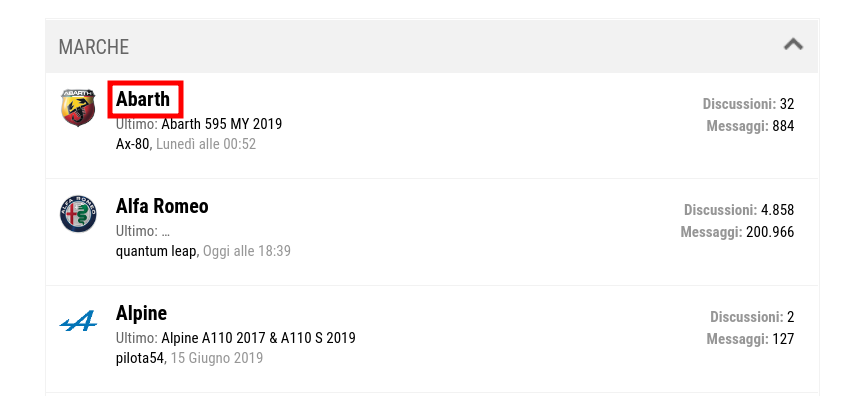
\includegraphics[width=\textwidth]{figures/screen/crawl/main-thematic-areas.png}
		\caption{Seed link corresponding to a base thematic area.}
		\label{fig:crawl-seed}
	\end{subfigure}
	\hfill
	\begin{subfigure}[ht]{0.8\textwidth}
		\centering
		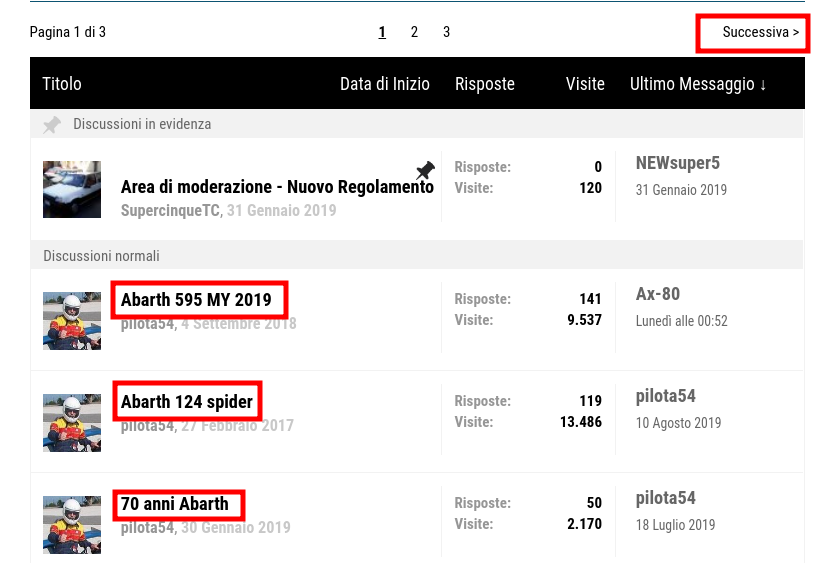
\includegraphics[width=\textwidth]{figures/screen/crawl/discussion-base.png}
		\caption{Base discussions link from previous seed link.}
		\label{fig:crawl-base-discussion}
	\end{subfigure}
	\hfill
	\begin{subfigure}[ht]{0.8\textwidth}
		\centering
		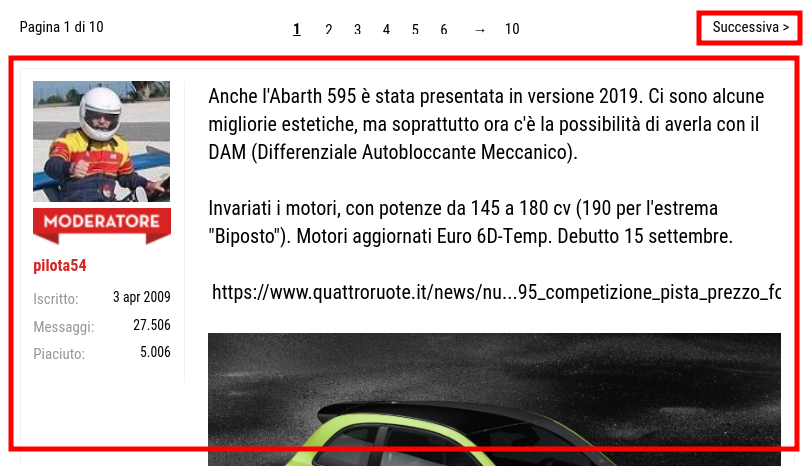
\includegraphics[width=\textwidth]{figures/screen/crawl/discussion.png}
		\caption{Discussion page.}
		\label{fig:crawl-discussion}
	\end{subfigure}
	\caption{Figurative example of forum crawling.}
	\label{fig:crawl}
\end{figure}

All information are then stored in a \ac{CSV} file in order to make simple the final annotation. Some numbers about the crawling process are shown in Table \ref{table:numbers-crawl}.

\begin{table}[ht]
	%\renewcommand{\arraystretch}{2.5}
	\centering
	\begin{tabular}{| c | c | c | c | } 
		\hline
		\textbf{Resource} & \textbf{\# Seeds} & \textbf{\# Discussions} & \textbf{\# Comments} \\ %[.2cm]
		\hline
		\hline
		Quattroruote & 57 & 37,721 & 181,065 \\ %[.2cm]
		\hline
		Autopareri & 51 & 15,803 & 552,364 \\ %[.2cm]
		\hline
		Bmwpassion & 5 & 4,011 & 75,482
		\\ %[.2cm]
		\hline
		Porschemania & 10 & 14,590 & 312,222 \\ %[.2cm]
		\hline
		Forumelettrico & 1 & 139 & 2,471 \\ %[.2cm]
		\hline
		HDmotori & 1 & 100 & 705 \\ %[.2cm]
		\hline
		\hline
		TOTAL & 125 & 72,364 & 1,124,309 \\ %[.2cm]
		\hline
	\end{tabular}
	\caption{Numbers about crawling process.}
	\label{table:numbers-crawl}
\end{table}

Manufacturer-free resources such as Quattroruote and Autopareri have been initialized with a seeds list made of manufacturers' base discussions page, while other resources such as Bmwpassion and HDmotori have been initialized searching for discussions related to Porsche.\\
As predictable, due to his blog nature, HDmotori is not discussion addicted, in fact it was possible to download just few comments.



\section{Dataset Annotation and Statistics}

The result of the crawling process is a \ac{CSV} file containing 1,124,309 comments. Some samples are shown in Tables \ref{tab:quattroruote-comment} \ref{tab:autopareri-comment} \ref{tab:bmwpassion-comment} \ref{tab:porschemania-comment} \ref{tab:forumelettrico-comment} \ref{tab:hdmotori-comment}.

\begin{table}[ht]
	\centering
	\begin{tabular}{l | l}
		Field & Value \\
		\hline 
		Thread & le foto delle nostre Alfa\\
		URL & \url{https://forum.quattroruote.it/threads/le-foto-delle...}\\
		Timestamp & 2012-05-22 00:00:00\\
		Author & valvonauta\_distratto\\
		Quote & La July e il Grigio (meglio tardi che mai...) Saluti\\
		Text & Non si vede un piffero : ? 
	\end{tabular}
	\caption{Quattroruote's sample comment}
	\label{tab:quattroruote-comment}
\end{table}

\begin{table}[ht]
	\centering
	\begin{tabular}{l | l}
		Field & Value \\
		\hline 
		Thread & Evo UK test: 599 \\
		URL & \url{https://www.autopareri.com/forums/topic/21814-evo...}\\
		Timestamp & 2007-01-30 20:48:34\\
		Author & poppy84\\
		Quote & \\
		Text & Adesso quanti ne avrebbe la 599... 550 ? 
	\end{tabular}
	\caption{Autopareri's sample comment}
	\label{tab:autopareri-comment}
\end{table}

\begin{table}[ht]
	\centering
	\begin{tabular}{l | l}
		Field & Value \\
		\hline 
		Thread & Dacia Logan MCV 7posti low cost \\
		URL & \url{https://www.bmwpassion.com/forum/threads/dacia...}\\
		Timestamp & 2004-08-23 00:00:00\\
		Author & mamo\\
		Quote & \\
		Text & Dopo la berlina la station wagon. La gamma della Dacia "Logan"\\& diventa più ampia con una versione più versatile e poliedrica.\\& Merito delle due ante incernierate ai lati che sostituiscono\\& il tradizionale portellone ma anche e soprattutto dell'allestimento\\& con due posti supplementari che rendono la "Logan MCV"\\& ( Multi Convivial Vehicle ) la più economica "sette posti" sul mercato.\\& D'altra parte i suoi punti di forza sono tutti concentrati nello spazio\\& sia per i passeggeri sia per i bagagli. Grazie al passo allungato di\\& una trentina di centimetri i due posti supplementari sono qualcosa\\& più che due "strapuntini" e il vano posteriore è pensato anche\\& per carichi rilevanti. Si va dai 500 litri della configurazione\\& "cinque passeggeri" ai 2350 di quella "due posti".\\& La meccanica ricalca quella della berlina con la novità di un "benzina"\\& 1600 con otto valvole ( 90 CV ) che affianca il 1400 ( 75 CV ) e il 1600\\& 16V da 105 CV. Unico il turbodiesel che è un "1500 dCi" da 68 CV.\\& I prezzi ( Ipt esclusa ) partono dagli 8950 euro della "1400" e\\& arrivano ai 12.350 della "1.5 dCi Lauréate". Per le "sette posti"\\& bisogna aggiungere 500 euro con un'unica avvertenza: questo\\& allestimento non è previsto sulle "1400". In arrivo nelle concessionarie\\& italiane a fine gennaio. quattroruote.it 
	\end{tabular}
	\caption{Bmwpassion's sample comment}
	\label{tab:bmwpassion-comment}
\end{table}

\begin{table}[ht]
	\centering
	\begin{tabular}{l | l}
		Field & Value \\
		\hline 
		Thread & Consiglio definitivo - premo il bottone rosso? \\
		URL & \url{http://www.porschemania.it/discus/messages/502415/...}\\
		Timestamp & 2012-12-21 17:36:00\\
		Author & alfi\\
		Quote & \\
		Text & ...qualche foto per renderci conto e darti un consiglio piu mirato ?  
	\end{tabular}
	\caption{Porschemania's sample comment}
	\label{tab:porschemania-comment}
\end{table}

\begin{table}[ht]
	\centering
	\begin{tabular}{l | l}
		Field & Value \\
		\hline 
		Thread & Colonnina EVAD Fast Municipio Sant'Ilario d'Enza \\
		URL & \url{https://www.forumelettrico.it/forum/colonnina-enel-fast-a-...}\\
		Timestamp & 2018-07-16 8:33:00\\
		Author & marco\\
		Quote & \\
		Text & Passato ieri e dopo settimane... la colonnina è ancora spenta \\&e davanti persiste l'installazione del palco. Per cui sposto la discussione\\& in abbandonate e speriamo che la colonnina possa presto venire\\& spostata ed avere maggior fortuna.
	\end{tabular}
	\caption{HDmotori's sample comment}
	\label{tab:forumelettrico-comment}
\end{table}

\begin{table}[ht]
	\centering
	\begin{tabular}{l | l}
		Field & Value \\
		\hline 
		Thread & Porsche Taycan: negli USA 3 anni di ricariche rapide incluse fino a 350 kW\\
		URL & \url{http://www.hdmotori.it/2019/01/29/porsche-taycan-3-anni...}\\
		Timestamp & 2019-01-29 10:46:00\\
		Author & luca bandini\\
		Quote & \\
		Text & arrivano arrivano... piuttosto tesla mi preoccupa perchè tutt'ora\\& non ha piani noti per sostituire la model S che ormai circola\\& da un po' di anni. a livello tecnico \\&è ottima per vendere dovranno modificare l'estetica ?  
	\end{tabular}
	\caption{HDmotori's sample comment}
	\label{tab:hdmotori-comment}
\end{table}


Just seeing few comments is possible to appreciate the heterogeneity of the texts. Some are very tight, like the one in Table \ref{tab:autopareri-comment}, or some are prolix like the on in Table \ref{tab:bmwpassion-comment}. Moreover, in some comments are present citations, while in others not. In general almost all comments are written using a colloquial language, in fact due to the informality of web forums are visible some writing mistakes, bad words and imprecations. Comments are full of technical details about the subject, also brands and models names are omnipresent. All these aspects are relevant, and sometimes fundamental, on sentiment classification.\\

At this point, the final phase to build the dataset consists on the actual sentiment classification. Sentences may express an unique sentiment polarity, or more generally diverse polarities about different topics. For instance the sentence "My car has awesome suspensions, but the engine is horrible" expresses a positive opinion about the car's mechanics, but a negative stance about the engine. For this reason it is important to catch sentiment position about every topic expressed in comments. From a first look on the forums about the most discussed topics, it comes that usual ones are:

\begin{itemize}
	\item Brand
	\item Interiors
	\item Exteriors
	\item Mechanics
	\item Performance
	\item Consumption/Fuel range
	\item Engine
	\item Electrical Mobility
	\item Off-road
	\item Onboard technology
	\item Maintenance
	\item Support/Concessionaires
\end{itemize}

For each comment it must be specified the sentiment polarity about every identified topic. For annotation it has been chosen a 5-degrees polarity: "very negative", "negative", "neutral", "positive" and "very positive", plus the additional "irrelevant" for topics that have not been mentioned. Moreover, together with the sentiment polarities, it must be also specified, if present and recognized, the manufacturer and the car model, and the overall sentiment of the comment without referring to any topic. Those last annotations have not been used for this work, but maybe in future works they comes useful, and now for free.\\
The total 1,124,309 crawled comments shuffled and divided into chunks of 250 comments each, in order to make possible the labeling involving crowdsourcing. The main reason of this choice comes from unavoidable deadlines and the need of a adequately large training dataset. Naturally the labeling of all the downloaded comments is unfeasible, so it has been decided a time window of one and an half month, with the purpose of labeling as much comments as possible. In total, have been involved about 20 people (most of them, because of obvious reasons, had labeled just one chunk of comments), to which it was provided a guide where it was specified the way to do the annotation in order to reduce as much as possible misunderstandings. In order to make the labeling simpler, faster and less affected by mispellings, it was provided an Excel sheet where were shown just useful information needed for taking the decision, and the label should be chosen using a dropdown menù. In case of "irrelevant" label, the cell should be left blank, in order to speed up the process. That made the labeling more user friendly than annotating directly on the CSV file. A screenshot of the Excel sheet is shown in Figure \ref{fig:excel-sheet}. At the end the total annotations count 7183 entries.\\


\begin{figure}[ht]
	\centering
	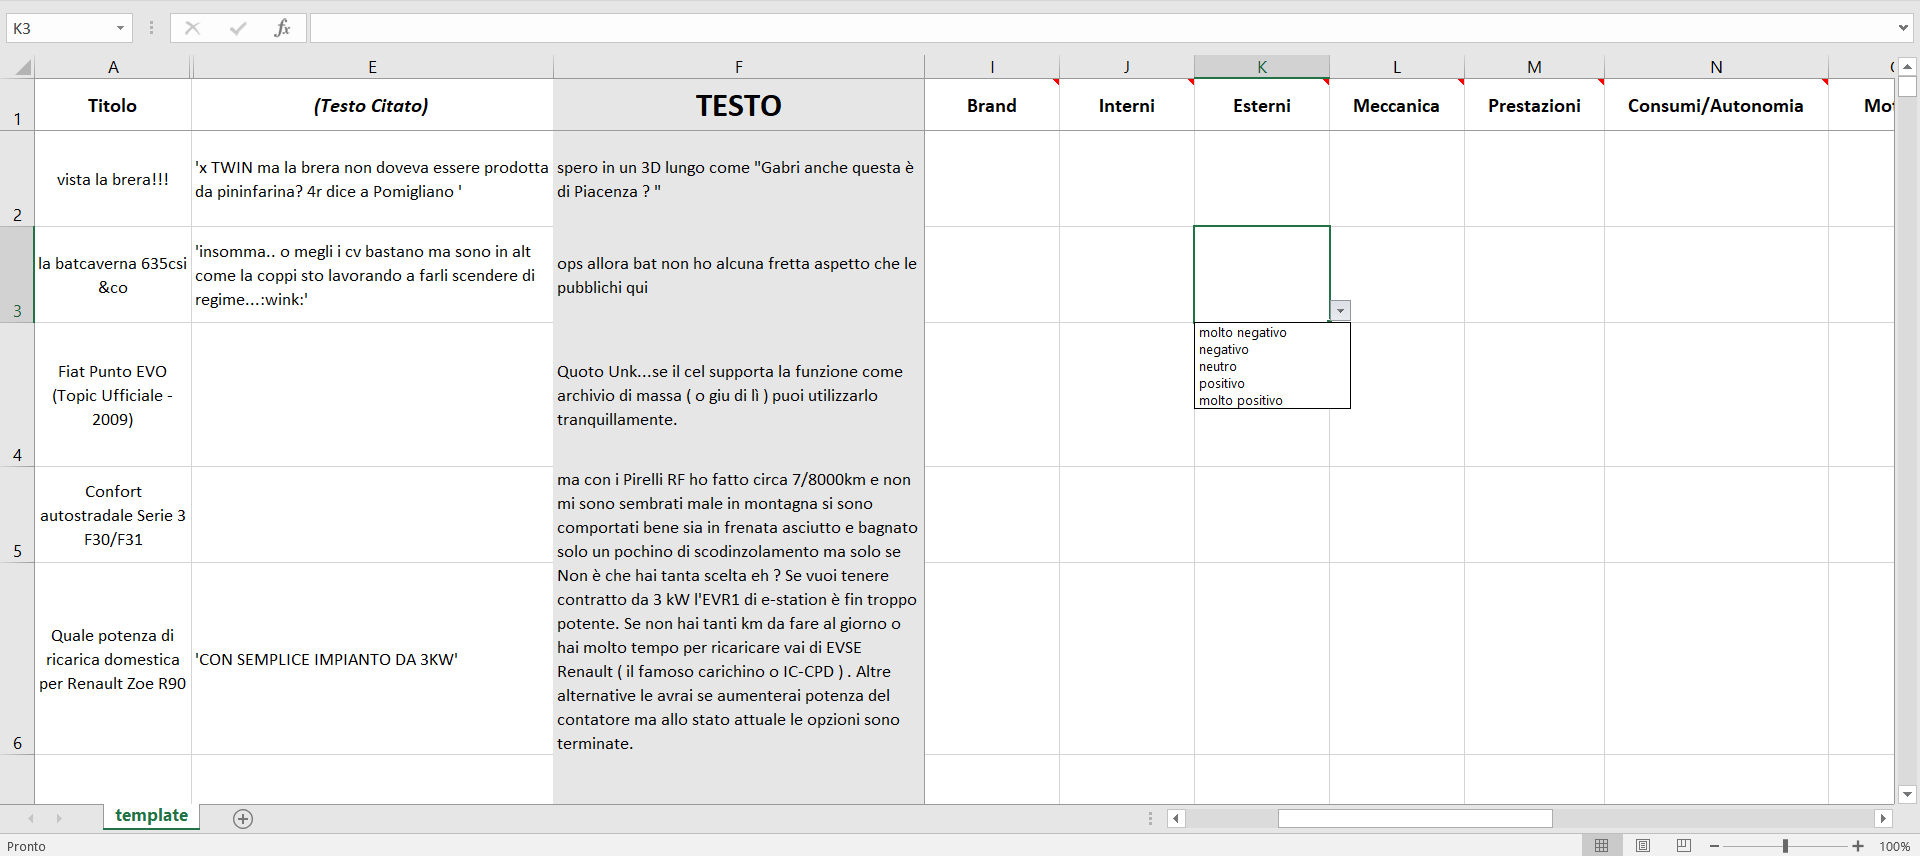
\includegraphics[width=1\textwidth]{figures/screen/excel-sheet.png}
	\caption{Graphical representation of an HTML DOM}
	\label{fig:excel-sheet}
\end{figure}


In general, detecting the stance of the user, from a comment, about a certain topic is not easy. Sometimes it is very clear like in this sample:

\begin{description}
	\item \textit{"Tranquillo il motore va molto bene anche in autostrada. Questa la mia recensione su S Cross stesso motore: https://forum.quattroruote.it/threads/recensione-s-cross-1-0-cool-2018.119763/\#post-2386072"}
\end{description}
where there is a clear evidence on positive polarity about the engine. Contrary, this sample it is not as easy to annotate:

\begin{description}
	\item \textit{"Ciao! presa oggi è uno spettacolo che la metà basta Solo un dubbio non riesco a trovare il modo di condividere la rubrica del mio Galaxy S2 con il coso della macchina dalle istruzioni non è che si capisca un granché bene qualcuno di quelli che l'ha presa ha idea di come si faccia con l'S2?"}
\end{description}
where there is a clear overall positive sentiment, but it is not expressed the topic. For cases like this, it comes the subjectivity of the annotator, for instance the positive sentiment may be referred to the exterior (since the car is "spectacular").
Other cases like this

\begin{description}
	\item \textit{"Per forza la tua Boxster è una giuletta taroccata Boxster!"}
\end{description}

present clearly a negative sentiment, but the topic it is not only unknown, but presumably there is not at all, so the annotation should be "irrelevant" for all categories. Other comments like

\begin{description}
	\item \textit{"Ciao!!! Fra Punto Evo ed Ibiza la qualità è a favore della seat perchè praticamente molti pezzi incluso il motore sono quelli della volkswagen. La carrozzeria il motore le sospensioni tutta l'elettronica... quindi non posso che consigliartela ad occhi chiusi. Riguardo ai consumi dubito fortemente che al primo pieno un 1.3 mjet possa aver fatto 21 km/litro.. come l'ha rilevato il consumo? Nel caso fosse vero allora sarebbe veramente un'ottima percorrenza.. Le doti che apprezzo di più della mia ibiza sono la tenuta di strada il cambio la linea e i consumi."}
\end{description}

present comparatives between two entities, in this case cars and engines. For these situations the rule was to take the decision with respect to the main reachable from the text or sometimes from the quote or the topic's title.\\

Below are shown some statistics about the outcome of the annotation's phase. Even if the labeling consists in a five-degrees of sentiment polarity, it was reduced into a three-degrees by grouping "very positive" into "positive" and "very negative" into "negative".
In Table \ref{table:annotations-distribution} are shown the actual number of annotations for each topic, that are visually represented in Figure \ref{fig:annotations}, while in Table \ref{table:annotations-distribution-perc-rel} are shown the percentages of the annotated sentiments referred to the total relevant ones (that are all but irrelevant). In Figure \ref{fig:annotations-relevant} are shown the distribution of sentiment polarities with respect to the relevant topics.


\begin{table}[H]
	\renewcommand{\arraystretch}{1.3}
	\centering
	\begin{tabular}{| c | c | c | c | c | c |} 
		\hline
		& \textbf{Positive} & \textbf{Neutral} & \textbf{Negative} & \textbf{Relevant} & \textbf{Not Relevant} \\ %[.03cm]
		\hline
		\hline
		\textbf{Brand}& 651 (9.06\%) & 280 (3.90\%) & 441 (6.14\%) & 1,372 (19.10\%) & 5,811 (80.90\%) \\ %[.06cm]
		\hline
		\textbf{Interiors}& 232 (3.23\%) & 116 (1.61\%) & 142 (1.98\%) & 490 (16.82\%) & 6,693  (93.18\%) \\ %[.06cm]
		\hline
		\textbf{Exteriors}& 424 (5.90\%) & 196 (2.73\%) & 246 (3.42\%) & 866 (12.05\%) & 6,317 (87.95\%) \\ %[.06cm]
		\hline
		\textbf{Mechanics}& 211 (2.94\%) & 279 (3.88\%) & 221 (3.08\%) & 711 (9.90\%) & 6,472 (90.10\%) \\ %[.06cm]
		\hline
		\textbf{Performance}& 258 (3.59\%) & 111 (1.55\%) & 121 (1.68\%) & 490 (6.82\%) & 6,693 (93.18\%) \\ %[.06cm]
		\hline
		\textbf{Consumption}& 121 (1.68\%) & 113 (1.57\%) & 87 (1.22\%) & 321 (4.47\%) & 6,862 (95.53\%) \\ %[.06cm]
		\hline
		\textbf{Engine}& 317 (4.41\%) & 358 (4.98\%) & 155 (2.16\%) & 830 (11.55\%) & 6,353 (88.45\%) \\ %[.06cm]
		\hline
		\textbf{Elec. Mobility}& 31 (0.43\%) & 96 (1.34\%) & 42 (0.58\%) & 169 (2.35\%) & 7,014 (97.65\%) \\ %[.06cm]
		\hline
		\textbf{Offroad}& 11 (0.15\%) & 6 (0.08\%) & 4 (0.06\%) & 21 (0.29\%) & 7,162 (99.71\%) \\ %[.06cm]
		\hline
		\textbf{Technology}& 117 (1.63\%) & 206 (2.87\%) & 134 (1.87\%) & 457 (6.37\%) & 6,726 (93.63\%) \\ %[.06cm]
		\hline
		\textbf{Maintenance}& 110 (1.53\%) & 252 (3.51\%) & 209 (2.91\%) & 571 (7.95\%) & 6,612 (92.05\%) \\ %[.06cm]
		\hline
		\textbf{Support}& 108 (1.50\%) & 178 (2.48\%) & 243 (3.38\%) & 529 (7.36\%) & 6,654 (92.64\%) \\ %[.06cm]
		\hline
		
	\end{tabular}
	\caption{Number of comments for every topic and sentiment polarity.}
	\label{table:annotations-distribution}
\end{table}

\begin{figure}[ht]
	\centering
	%	\begin{subfigure}{1\textwidth} % width of left subfigure
	%		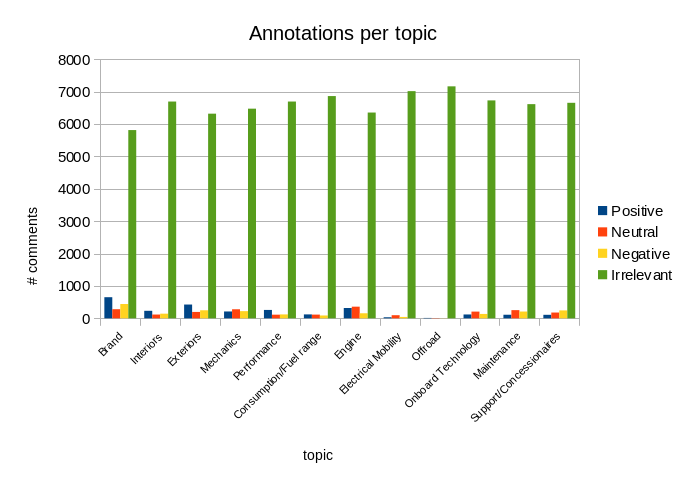
\includegraphics[width=1\textwidth]{figures/charts/annotations-distribution.png}
	%		%\caption{Graphical representation of an HTML DOM}
	%		\label{fig:annotations-distribution}
	%	\end{subfigure}
	%	\vspace{-1cm} % here you can insert horizontal or vertical space
	\begin{subfigure}{1\textwidth} % width of right subfigure
		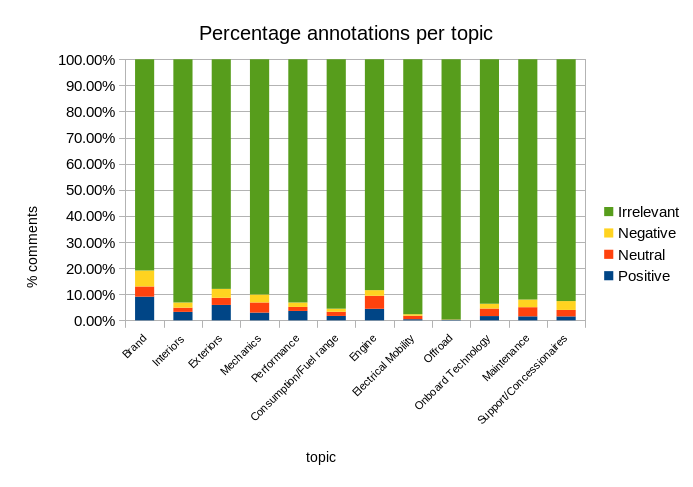
\includegraphics[width=1\textwidth]{figures/charts/annotations-distribution-perc.png}
		%\caption{Graphical representation of an HTML DOM}
		\label{fig:annotations-distribution-perc}
	\end{subfigure}
	\caption{Labels' distribution} % caption for whole figure
	\label{fig:annotations}
\end{figure}

%\begin{table}[ht]
%	\renewcommand{\arraystretch}{1.5}
%	\centering
%	\begin{tabular}{| c | c | c | c | c |} 
%		\hline
%		& \textbf{\% Positive} & \textbf{\% Neutral} & \textbf{\% Negative} & \textbf{\% Irrelevant} \\ [.06cm]
%		\hline
%		\hline
%		\textbf{Brand}& 9.06\% & 3.90\% & 6.14\% & 80.90\% \\ [.06cm]
%		\hline
%		\textbf{Interiors}& 3.23\% & 1.61\% & 1.98\% & 93.18\% \\ [.06cm]
%		\hline
%		\textbf{Exteriors}& 5.90\% & 2.73\% & 3.42\% & 87.95\%  \\ [.06cm]
%		\hline
%		\textbf{Mechanics}& 2.94\% & 3.88\% & 3.08\% & 90.10\% \\ [.06cm]
%		\hline
%		\textbf{Performance} & 3.59\% & 1.55\% & 1.68\% & 93.18\% \\ [.06cm]
%		\hline
%		\textbf{Consumption} & 1.68\% & 1.57\% & 1.22\% & 95.53\% \\ [.06cm]
%		\hline
%		\textbf{Engine}& 4.41\% & 4.98\% & 2.16\% & 88.45\% \\ [.06cm]
%		\hline
%		\textbf{Electrical Mobility} & 0.43\% & 1.34\% & 0.58\% & 97.65\% \\ [.06cm]
%		\hline
%	\textbf{Technology} & 1.63\% & 2.87\% & 1.87\% & 93.63\% \\ [.06cm]
%		\hline
%		\textbf{Maintenance} & 1.53\% & 3.51\% & 2.91\% & 92.05\% \\ [.06cm]
%		\hline
%		\textbf{Support} & 1.50\% & 2.48\% & 3.38\% & 92.64\% \\ [.06cm]
%		\hline
		
%	\end{tabular}
%	\caption{Percentage distribution of comments for every topic and sentiment polarity.}
%	\label{table:annotations-distribution-perc}
%\end{table}





\begin{table}[ht]
	\renewcommand{\arraystretch}{1.3}
	\centering
	\begin{tabular}{| c | c | c | c | c |} 
		\hline
		& \textbf{\# Relevant} & \textbf{\% Positive} & \textbf{\% Neutral} & \textbf{\% Negative} \\ [.06cm]
		\hline
		\hline
		\textbf{Brand}& 1,372 & 47.45\% & 20.41\% & 32.14\% \\ %[.06cm]
		\hline
		\textbf{Interiors}& 490 & 47.35\% & 23.67\% & 28.98\% \\ %[.06cm]
		\hline
		\textbf{Exteriors}& 866 & 48.96\% & 22.63\% & 28.41\%  \\% [.06cm]
		\hline
		\textbf{Mechanics}& 711 & 29.68\% & 39.24\% & 31.08\% \\ %[.06cm]
		\hline
		\textbf{Performance}& 490 & 52.65\% & 22.65\% & 24.70\% \\ %[.06cm]
		\hline
		\textbf{Consumption}& 321 & 37.70\% & 35.20\% & 27.10\% \\ %[.06cm]
		\hline
		\textbf{Engine}& 830 & 38.20\% & 43.13\% & 18.67\% \\ %[.06cm]
		\hline
		\textbf{Electrical Mobility}& 169 & 18.35\% & 56.80\% & 24.85\% \\% [.06cm]
		\hline
		\textbf{Offroad}& 21 & 52.38\% & 28.57\% & 19.05\% \\ %[.06cm]
		\hline
		\textbf{Technology}& 457 & 25.60\% & 45.08\% & 29.32\% \\ %[.06cm]
		\hline
		\textbf{Maintenance}& 571 & 19.26\% & 44.14\% & 36.60\% \\ %[.06cm]
		\hline
		\textbf{Support}& 529 & 20.42\% & 33.65\% & 45.93\% \\ %[.06cm]
		\hline
		
	\end{tabular}
	\caption{Percentage distribution of comments for every topic and sentiment polarity.}
	\label{table:annotations-distribution-perc-rel}
\end{table}


\begin{figure}[ht]
	\centering
	\begin{subfigure}{1\textwidth} % width of left subfigure
		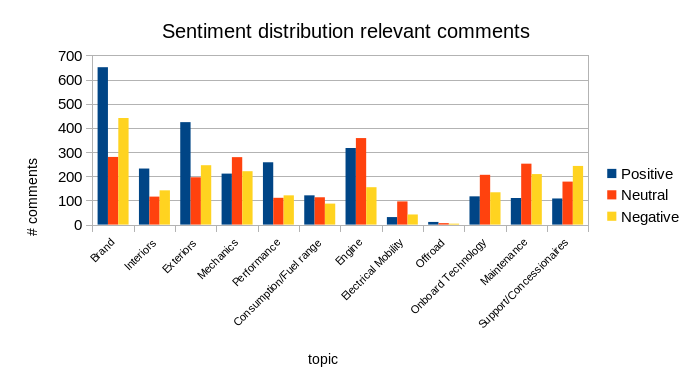
\includegraphics[width=1\textwidth]{figures/charts/sentiment-distribution.png}
		%\caption{Graphical representation of an HTML DOM}
		\label{fig:sentiment-distribution}
	\end{subfigure}
		\vspace{-1cm} % here you can insert horizontal or vertical space
	\begin{subfigure}{1\textwidth} % width of right subfigure
		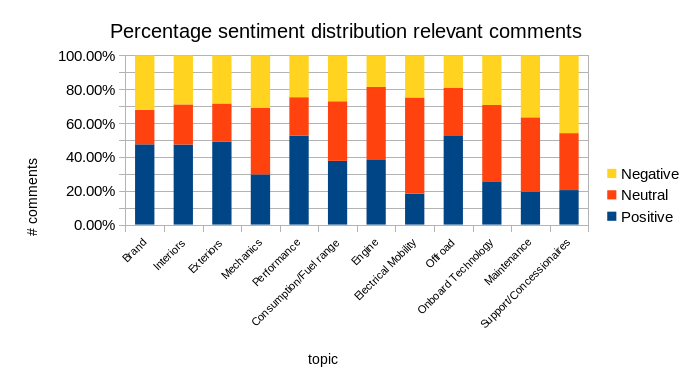
\includegraphics[width=1\textwidth]{figures/charts/sentiment-distribution-perc.png}
	\label{fig:sentiment-distribution-perc}
	\end{subfigure}
	\caption{Sentiment polarity distribution per topic for relevant ones} % caption for whole figure
	\label{fig:annotations-relevant}
\end{figure}


As predicable, every class has the majority on "irrelevant" label, which is absolutely right since there are lot of comments that give not information about any category, and then other comments usually contain just one or a couple of different topics, so in all others they are labeled as "irrelevant". From the statistics comes some mispredictions, in fact initially the class "offroad" was thought as a topic that is commonly touched, but actually it is not at all. \\
From the graphics it is possible to see that the most discussed topics are "brand", "interiors", "exteriors", "engine" and "maintenance", while the less touched are "offroad" (as just said) and "electrical mobility". For what concerns "electrical mobility" topic the point is that it is a new frontier related to innovation, but forums contain decades of "legacy" mobility, so it is not so strange.\\
A few interesting observation can be made looking for the bar-charts in Figure \ref{fig:annotations-relevant}: recalling what said about unbalances in Twitter Sentiment Analysis' datasets, here it comes the same issue, in fact most of the topics present visible unbalance, but without an overall preferred polarity. From these statistics it is possible to make supposition about the trends in automotive forums (obviously supposing the dataset is representative): when a brand is mentioned is mostly for praise it, but in general are touched the ends polarities. Moreover, an unsurprising outcomes regards the topics "maintenance" and "support/concessionaires": they show a majority on negatives above positives, and it is explicable since breakages are essentially bad experiences, and so it has repercussions on the comments. And also, if in a car is all fine, presumably there is no motivation to write a comment about maintenance.\\

What seen is a snapshot of the environment where the sentiment analysis algorithm is supposed to run. The following phase consists on the thinking out a domain specific sentiment analysis algorithm.




























